\documentclass[a4paper,12pt]{article}
\usepackage{graphicx} % Required for inserting images
\usepackage{xcolor}
\usepackage{polski}
\usepackage{multicol}
\usepackage{url}
\usepackage[hmargin=1cm,vmargin=2cm]{geometry}

\title{Projekt Telekomunikacja}
\author{Jakub Zając, Marcin Klocek}
\date{December 2024}

\begin{document}

\maketitle

\section{Opis projektu}
W ramach projektu została opracowana gra Kółko i Krzyżyk. W grze może wziąć udział dwóch graczy spośród których jeden jest serwerem, drugi klientem. Po nawiązaniu połączenia, następuje przekazanie kluczy publiczbych przez obie strony co zapewnia symetryczne szyfrowanie (TLS RSA). Następuje rozgrywka. Dane wymieniane są za pomocą protokołu TCP/IP. Użyty język programowania: \textbf{Python 3} wraz z systemem wersjonowania \textit{git}.

\section{RSA/Padding OAEP \color{red} Autor: Jakub Zając }
\subsection{RSA}
Do szyfrowania użyty został protokół RSA z kluczem 1024-bitowy. Zgodnie ze specyfikacją algorymtu szyfrowanie zostaje przeprowadzane poprzez mnożenie modularne: \newline

\begin{multicols}{2}
\begin{center}
\Large Szyfrowanie \newline
\Large $ c~=~m^e~\mathrm{mod} ~ n$
\end{center}
\vfill

\begin{center}
\Large Deszyfrowanie \newline
\Large $ m~=~c^d~\mathrm{mod} ~ n$
\end{center}
\vfill
\end{multicols}
Gdzie \textit{c}= wiadomość zaszyfrowana w postaci liczby całkowitej z zakresu  1 $\cdots$ \textit{n}, gdzie n to liczba większa od $2^{1023-1}$, \textit{e} - klucz publiczny oraz \textit{d} klucz prywatny. Program za każdym razem losuje dwie liczby pierwsze wystarczająco duże by ich iloczyn dał w wyniku liczbe \textit{n}. Trudność złamania szyfry polega na trudności faktoryzacji \textit{n}.

\newpage
\subsection{Padding}
Aby zapewnić danym odpowiednią długość (przy zbyt małej długości bitowej danych szyfr może zostać łatwo złamany) stisujemy \textit{Optimal asymmetric encryption padding}, który odpowiednio wydłuży dane. Algorymt ten wykorzystuje hashowanie \textbf{SHA-256}  oraz funkcje \textbf{mgf1}. Dodatkowo każdorazowo przy padding'owniu losowany jest nowy \textit{seed} używany podczas tego procesu. W naszym projekcie użyłem gotowych bibliotecznych funkcji hashujących oraz gotowej implmentacji funkcji \textbf{mgf1}.

\begin{figure}
\centerline{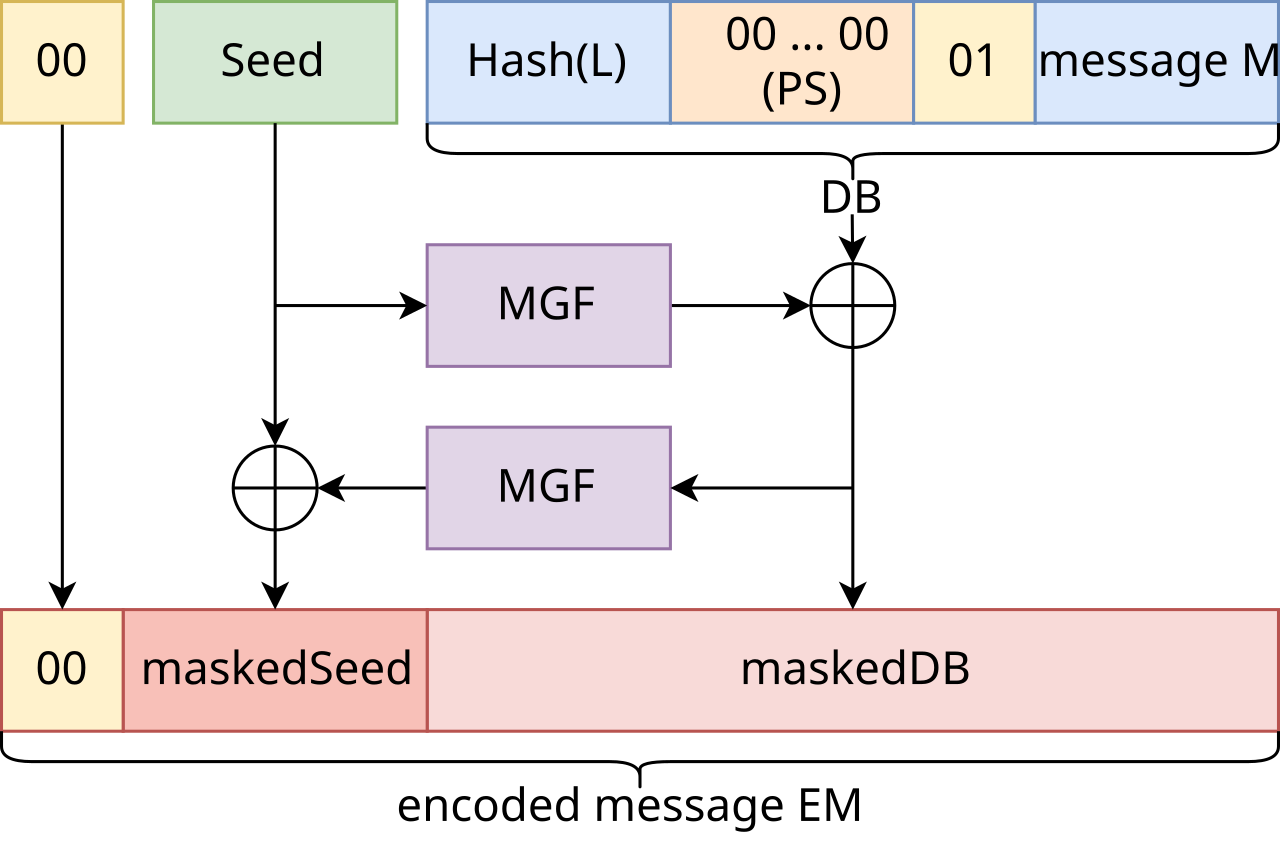
\includegraphics[scale=0.15]{OAEP.png}}
\caption{Optimal asymmetric encryption padding}
\end{figure}
Całkowita długość ramki to 128 bajtów, funkcja hashująca koduje pusty label = '' do porcji 32 bajtowej, \textit{seed} również ma 32 bajty, resza to wiadomość oraz uzupełnienia tak jak to widać na rysunku. Wynikowo dane mają 1024 znaki bitowe. Operacja z krzyżykiem w kole to bitowe XOR.

\section{Komunikacja SerwerClient \color{red} Autorzy: Jakub Zając, ... }
Komunikacja nawiązywana jest poprzez gniazdo (\textit{socket}) za pomocą protokołu IP. Po nawiązaniu połączenia serwer-client, następuje podwójna wymiana kluczy. Zarówno klient jak i serwer ma swoją parę kluczy publicznych \textit{(d,e)} którą wymienia między sobą w przestrzeni publicznej , dzięki czemu szyfrowanie działa w obie strony.  

\begin{figure}
\centerline{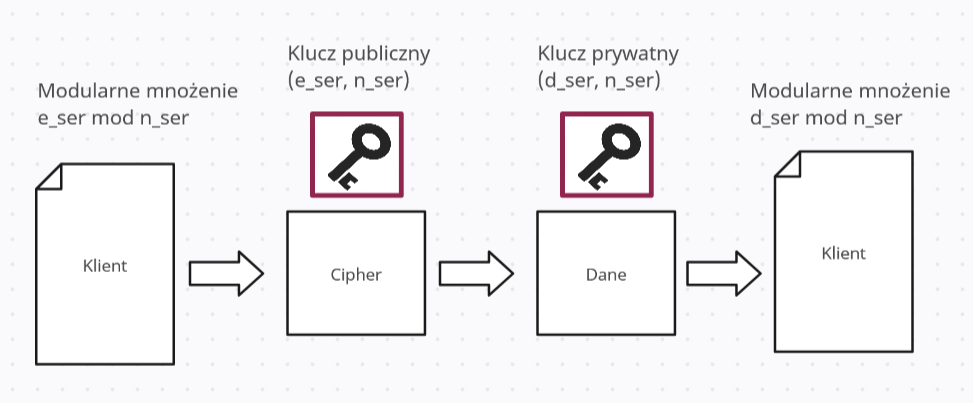
\includegraphics[scale=0.6]{Raport/ProceszSzyfrowania.png}}
\caption{Szyfrowanie Serwer-Klient. W drugą stronę przebiega identycznie.}
\end{figure}

Nawiązanie połączenia następuje w 4 stanach: 
\begin{enumerate}
\item \textbf{PUBLIC\_KEY\_EXCHANGE\_SERVER} - udostępnienie klucza przez serwer  \item \textbf{CLIENT\_KEY\_ACK} - potwierdzenie klienta \item \textbf{PUBLIC\_KEY\_EXCHANGE\_CLIENT} - udostępnienie klucza przez klienta  \item \textbf{SERVER\_KEY\_ACK} - potwierdzenie serwera  
\item \textbf{COMMUNICATION} - rozpoczęcie właściwej komunikacji.
\end{enumerate}
W projekcie używany jest \textbf{socket.socket(socket.AF\_INET, socket.SOCK\_STREAM)} udostępniany w standardowej bibliotece. Jest to protokół TCP/IPv4.






\section{Repozytorium}
Poniżej udostępniamy link do naszego repozytorim ze wszystkimi kodami źródłowymi.
\newline
\url{https://github.com/mklck/tt-project/tree/main}
\end{document}
